\documentclass[a4paper,12pt]{article}


%%% Работа с русским языком
\usepackage{cmap}					% поиск в PDF
\usepackage{mathtext} 				% русские буквы в формулах
\usepackage[T2A]{fontenc}			% кодировка
\usepackage[utf8]{inputenc}			% кодировка исходного текста
\usepackage[english,russian]{babel}	% локализация и переносы
\usepackage{indentfirst}
\frenchspacing

\newcommand{\vyp}{\ensuremath{\hookrightarrow}}
\renewcommand{\epsilon}{\ensuremath{\varepsilon}}
\renewcommand{\phi}{\ensuremath{\varphi}}
\renewcommand{\kappa}{\ensuremath{\varkappa}}
\renewcommand{\le}{\ensuremath{\leqslant}}
\renewcommand{\leq}{\ensuremath{\leqslant}}
\renewcommand{\ge}{\ensuremath{\geqslant}}
\renewcommand{\geq}{\ensuremath{\geqslant}}
\renewcommand{\emptyset}{\varnothing}
\newcommand{\Ra}{\ensuremath{\Rightarrow}}
\newcommand{\ra}{\ensuremath{\rightarrow}}
\newcommand{\LRa}{\ensuremath{\Leftrightarrow}}
\newcommand{\tbf}{\textbf}
\newcommand{\ov}{\ensuremath{\overline}}
\newcommand{\CC}{\ensuremath{\mathbb{C}}}
\newcommand{\RR}{\ensuremath{\mathbb{R}}}
\newcommand{\NN}{\ensuremath{\mathbb{N}}}
\newcommand{\QQ}{\ensuremath{\mathbb{Q}}}
\newcommand{\ZZ}{\ensuremath{\mathbb{Z}}}

%%% Дополнительная работа с математикой
\usepackage{amsmath,amsfonts,amssymb,amsthm,mathtools} % AMS
\usepackage{icomma} % "Умная" запятая: $0,2$ --- число, $0, 2$ --- перечисление

%% Номера формул
%\mathtoolsset{showonlyrefs=true} % Показывать номера только у тех формул, на которые есть \eqref{} в тексте.
%\usepackage{leqno} % Нумереация формул слева

%% Свои команды
\DeclareMathOperator{\sgn}{\mathop{sgn}}

%% Перенос знаков в формулах (по Львовскому)
\newcommand*{\hm}[1]{#1\nobreak\discretionary{}
{\hbox{$\mathsurround=0pt #1$}}{}}



%%% Работа с картинками
\usepackage{graphicx}  % Для вставки рисунков
\graphicspath{{images/}{images2/}}  % папки с картинками
\setlength\fboxsep{3pt} % Отступ рамки \fbox{} от рисунка
\setlength\fboxrule{1pt} % Толщина линий рамки \fbox{}
\usepackage{wrapfig} % Обтекание рисунков текстом

%%% Работа с таблицами
\usepackage{array,tabularx,tabulary,booktabs} % Дополнительная работа с таблицами
\usepackage{longtable}  % Длинные таблицы
\usepackage{multirow} % Слияние строк в таблице

%%% Теоремы
\theoremstyle{plain} % Это стиль по умолчанию, его можно не переопределять.
\newtheorem{theorem}{Теорема}[section]
\newtheorem{proposition}[theorem]{Утверждение}
 
\theoremstyle{definition} % "Определение"
\newtheorem{corollary}{Следствие}[theorem]
\newtheorem{problem}{Задача}[section]
 
\theoremstyle{remark} % "Примечание"
\newtheorem*{nonum}{Решение}

%%% Программирование
\usepackage{etoolbox} % логические операторы

%%% Страница
\usepackage{extsizes} % Возможность сделать 14-й шрифт
\usepackage{geometry} % Простой способ задавать поля
	\geometry{top=20mm}
	\geometry{bottom=20mm}
	\geometry{left=5mm}
	\geometry{right=15mm}
 %
\usepackage{fancyhdr} % Колонтитулы
 	\pagestyle{fancy}
 	\renewcommand{\headrulewidth}{1pt}  % Толщина линейки, отчеркивающей верхний колонтитул
%\fancypagestyle{firstpage}{
	\rhead{\large{Исыпов Илья}}
%}
% 	\lfoot{Нижний левый}
% 	\rfoot{\large{Рябых Владислав, Б05-905}}
% 	\rhead{Верхний правый]}
% 	\chead{Верхний в центре}
 	\lhead{\large{Рябых Владислав}}
%	\cfoot{Нижний в центре} % По умолчанию здесь номер страницы

\usepackage{setspace} % Интерлиньяж
\onehalfspacing % Интерлиньяж 1.5
%\doublespacing % Интерлиньяж 2
%\singlespacing % Интерлиньяж 1

\usepackage{lastpage} % Узнать, сколько всего страниц в документе.

\usepackage{soul} % Модификаторы начертания

\usepackage{hyperref}
\usepackage[usenames,dvipsnames,svgnames,table,rgb]{xcolor}
\hypersetup{				% Гиперссылки
    unicode=true,           % русские буквы в раздела PDF
    pdftitle={Заголовок},   % Заголовок
    pdfauthor={Автор},      % Автор
    pdfsubject={Тема},      % Тема
    pdfcreator={Создатель}, % Создатель
    pdfproducer={Производитель}, % Производитель
    pdfkeywords={keyword1} {key2} {key3}, % Ключевые слова
    colorlinks=true,       	% false: ссылки в рамках; true: цветные ссылки
    linkcolor=red,          % внутренние ссылки
    citecolor=black,        % на библиографию
    filecolor=magenta,      % на файлы
    urlcolor=cyan           % на URL
}

\usepackage{csquotes} % Еще инструменты для ссылок

%\usepackage[style=authoryear,maxcitenames=2,backend=biber,sorting=nty]{biblatex}

\usepackage{multicol} % Несколько колонок

\usepackage{tikz} % Работа с графикой
\usepackage{pgfplots}
\usepackage{pgfplotstable}

\usepackage{caption}
\long\def\comment{}
\setlength{\abovecaptionskip}{7pt}
\setlength{\belowcaptionskip}{7pt}
\mathtoolsset{showonlyrefs}


\begin{document}

\begin{titlepage}
	\begin{center}
		
		\textsc{\LARGE Московский\\[-0.2cm]Физико-Технический Институт\\[0.1cm]\large (национальный исследовательский университет)}\\[1.5cm] 
		
	
\includegraphics[width=0.3\textwidth]{hv_s_no_bg.png}~\\[1cm]

	\textsc{\Large Оптика. \\ Лабораторный практикум. }\\[0.2cm]

	% Title
	\HRule \\[0.4cm]
	{ \LARGE \bfseries Лабораторная работа № 4.4.1 \\ Амплитудная дифракционная решётка \\[0.4cm] }

	\HRule \\[1.5cm]
		
		% Author and supervisor
		\noindent
		\begin{minipage}{0.4\textwidth}
			\begin{flushleft} \large
			\end{flushleft}
		\end{minipage}%
		\begin{minipage}{0.4\textwidth}
			\begin{flushright} \large
			\end{flushright}
		\end{minipage}
		
		
		\large{\begin{flushright}
				\vfill
				\textbf{Выполнили}:\\
				\textbf{Рябых Владислав,\\}
				\textbf{Исыпов Илья\\}
				\textbf{группа Б05-905}
		\end{flushright}}
		
		
		{\large \today}\\
		
		
	\end{center}
\end{titlepage}

\subsubsection*{Цель работы:}знакомство с работой и настройкой гониометра Г5, определение спектральных характеристик амплитудной решетки.

\subsubsection*{Оборудование:} гониометр, дифракционная решетка, ртутная лампа. 

\section*{Теория}

\begin{wrapfigure}[15]{L}{0.5\linewidth}
	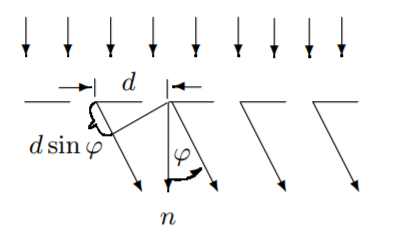
\includegraphics[scale = 0.9]{img1}
	\caption{дифракция световых волн на решётке}
\end{wrapfigure}

Амплитудную решетку можно представить в виде непрозрачного экрана, в котором прорезано большое число $N$ параллельных щелей - штрихов, расстояние между которыми $d$ (шаг или период решетки).

Пусть на решетку падает излучение с длиной волны $\lambda$ по нормали к плоскости решетки. Вследствие дифракции лучи, прошедшие через щель в решетке, отклоняются от своего первоначального направления. Рассмотрим лучи, отклонившиеся на угол $\varphi$. Разность хода лучей о эквивалентных точек двух соседних штрихов равна 
\begin{equation}
	\Delta = d \sin \varphi .
	\label{eq:dif1}
\end{equation}

\noindent Если эта величина равна целому числу длин волны:
\begin{equation}
	d \sin \varphi = m \lambda, \quad m = 0, \pm 1, \pm 2, ... ,
	\label{eq:dif2}
\end{equation}

\noindent то волны взаимно усиливают друг друга.\\

В соответствии с принципом Гюйгенса–Френеля распределение интенсивности в дифракционной картине определяется суперпозицией волн, приходящих в точку наблюдения от различных щелей решётки. При этом амплитуды всех интерферирующих волн при заданном угле $\varphi$ практически одинаковы, а фазы составляют арифметическую прогрессию.

\begin{equation}
	I = I_0 \dfrac{sin^2[N(kd \sin{\varphi})/2]}{sin^2[(kd \sin{\varphi})/2]},
	\label{eq:dif3}
\end{equation}

\noindent где $k$~--~волновое число, $I_0$~--~интенсивность волны, идущей от одного штриха. \\

При большом числе щелей свет, прошедший через решётку, распространяется по ряду резко ограниченных направлений. Если на дифракционную решётку падает свет сложного спектрального состава, то после решётки образуется спектр, причём фиолетовые лучи отклоняются решёткой меньше, чем красные (чем больше длина волны, тем сильнее лучи отклоняются решеткой).

\begin{wrapfigure}[12]{R}{0.5\linewidth}
	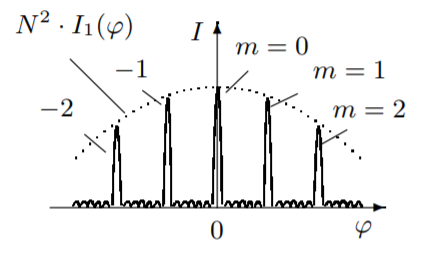
\includegraphics[scale = 0.7]{img2}
	\caption{распределение интенсивности света при дифракции Фраунгофера на решётке}
\end{wrapfigure}

\noindent Входящая в формулу $\eqref{eq:dif1}$ величина $m$ носит название \textit{порядка спектра}. При $m = 0$ максимумы интенсивности для всех длин волн располагаются при $\varphi = 0$ и накладываются друг на друга. При освещении белым светом нулевой максимум, в отличие от всех прочих, оказывается поэтому неокрашенным. Спектры первого, второго и т.д. порядков располагаются симметрично по обе стороны от нулевого.

\subsubsection*{Угловая дисперсия}

\noindent \textit{Угловая дисперсия} $D$ характеризует угловое расстояние $d \varphi$ между спектральными линиями, отстоящими по длине волны на $d \lambda$:

\begin{equation}
	D=\dfrac{d \varphi}{d \lambda}=\frac{m}{d cos \varphi}=\dfrac{m}{\sqrt{d^{2}-(m \lambda)^{2}}}
	\label{eq:dif4}
\end{equation}

\subsubsection*{Разрешающая способность дифракционной решетки}

\begin{wrapfigure}[16]{L}{0.45\linewidth}
	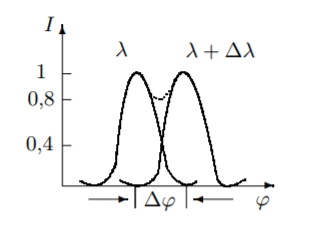
\includegraphics[scale = 1]{img3}
	\caption{к определению разрешающей способности дифракционной решётки}
\end{wrapfigure}

\noindent Возможность разрешения двух близких спектральных линий зависит от их ширины и от расстояния между ними. Угловое расстояние между двумя близкими спектральными компонентами с длинами волн $\lambda$ и ($\lambda + \Delta \lambda$) равно:

\begin{equation}
	\Delta \varphi =  D d \lambda = \frac{m \Delta \lambda}{d \cos{\varphi}}.
	\label{eq:dif5}
\end{equation}

\noindent Согласно критерию Рэлея линии становятся неразличимыми, когда расстояние между ними меньше, чем расстояние от максимума одной линии до её первого минимума. Пусть решетка имеет $N$ штрихов. Выберем главный максимум $m$-го порядка для компоненты $\lambda$. Направление на первый дифракционный минимум дается равенством 
\[ d \sin \varphi = \left( m + \dfrac{1}{N} \right) \lambda. \]
По критерию Рэлея это же направление должно соответствовать главному дифракционному максимуму для второй компоненты $\lambda + \Delta \lambda$:
\[ d \sin \varphi = m (\lambda + \Delta \lambda) .\]
Из последних двух равенств находим 
\begin{equation}
	\Delta \lambda = \dfrac{\lambda}{mN}.
	\label{eq:dif6}
\end{equation}
По определению \textit{разрешающая способность спектрального прибора} $R = \lambda / \Delta \lambda$~--~это отношение длины волны к разности длин волн двух линий, разрешаемых по критерию Рэлея.

\noindent Таким образом, приходим к следующему выражению для разрешающей способности дифракционной решетки:
\begin{equation}
	R = \lambda / \Delta \lambda = mN.
	\label{eq:dif7}
\end{equation}

\subsubsection*{Дисперсионная область}

\noindent При достаточно широком спектральном интервале падающего света спектры разных порядков могут накладываться друг на друга. Предельная ширина спектрального интервала $\Delta \lambda$, при которой спектры соседних порядков $(m$ и $m + 1)$ перекрываются только
своими границами, называется \textit{дисперсионной областью} $G$. При этом

\[d \sin\varphi = m(\lambda + \Delta \lambda ) = (m + 1)\lambda \]

\noindent и дисперсионная область

\begin{equation}
	G = \Delta \lambda = \frac{\lambda}{m}.
	\label{eq:dif8}
\end{equation}

\subsubsection*{Экспериментальная установка}

\begin{figure}[h]
	\centering
	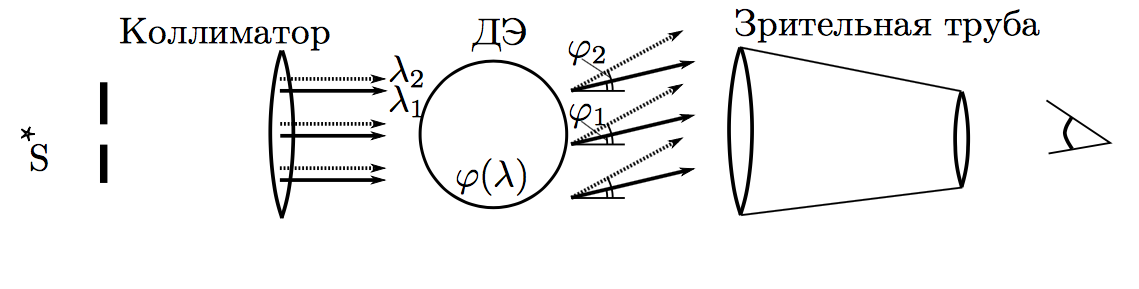
\includegraphics[scale = 0.4]{scheme}
	\caption{схема прибора: источник-коллиматор -- диспергирующий элемент -- зрительная труба}
	\label{fig:scheme}
\end{figure}

\noindent Исследование спектра ртутной лампы, определение периода и спектральных характеристик решетки проводится с помощью гониометра Г5.
\newpage

\section*{Ход работы}

\begin{enumerate}
	\item Подберем ширину входной щели коллиматора так, чтобы ширина линий жёлтого дублета была чуть больше промежутка между линиями двойного штриха окуляра зрительной трубы. Установим высоту щели, удобную для измерений. Измерим угловые координаты спектральных линий ртути для $\pm 1$ порядка
	
	\begin{table}[bhtp!]
		\begin{center}
			\begin{tabular}{|c|c|c|c|c|c|}
				\hline
				Порядок & Цвет & $\lambda, \nm$   & $\varphi$   & $\sin \varphi $  & $\delta (\sin \varphi)$\\ \hline
				1       & Фиолетовый & 404.7 & \ang{168;22;18} & 0.202  & 0.0012 \\ \hline
				1       & Синий      & 435.8 & \ang{167;26;54} & 0.217  & 0.0013 \\ \hline
				1       & Голубой    & 491.6 & \ang{165;48;54} & 0.245  & 0.0015 \\ \hline
				1       & Зеленый    & 546.1 & \ang{164;12;08} & 0.272  & 0.0016 \\ \hline
				1       & Желтый 1   & 577   & \ang{163;16;22} & 0.288  & 0.0017 \\ \hline
				1       & Желтый 2   & 579.1 & \ang{163;12;12} & 0.289  & 0.0018 \\ \hline
				-1      & Фиолетовый & 404.7 & \ang{191;40;32} & -0.202 & 0.0012 \\ \hline
				-1      & Синий      & 435.8 & \ang{192;32;32} & -0.217 & 0.0013 \\ \hline
				-1      & Голубой    & 491.6 & \ang{194;12;58} & -0.246 & 0.0015 \\ \hline
				-1      & Зеленый    & 546.1 & \ang{195;50;50} & -0.273 & 0.0017 \\ \hline
				-1      & Желтый 1   & 577   & \ang{196;45;09} & -0.288 & 0.0017 \\ \hline
				-1      & Желтый 2   & 579.1 & \ang{196;48;55} & -0.289 & 0.0018 \\ \hline
			\end{tabular}
			\caption{угловые координаты спектральных линий ртути для $\pm 1$ порядка}
			\label{tabular:graph1}
		\end{center}
	\end{table}
	
	
	\noindent По полученным данным таблицы $\ref{tabular:graph1}$ построим график зависимости $\sin \varphi (\lambda)$ для разных порядков: рис. $\ref{1st}$ и рис. $\ref{-1st}$


\begin{center}
	\begin{figure}[bhtp!]
		\centering
		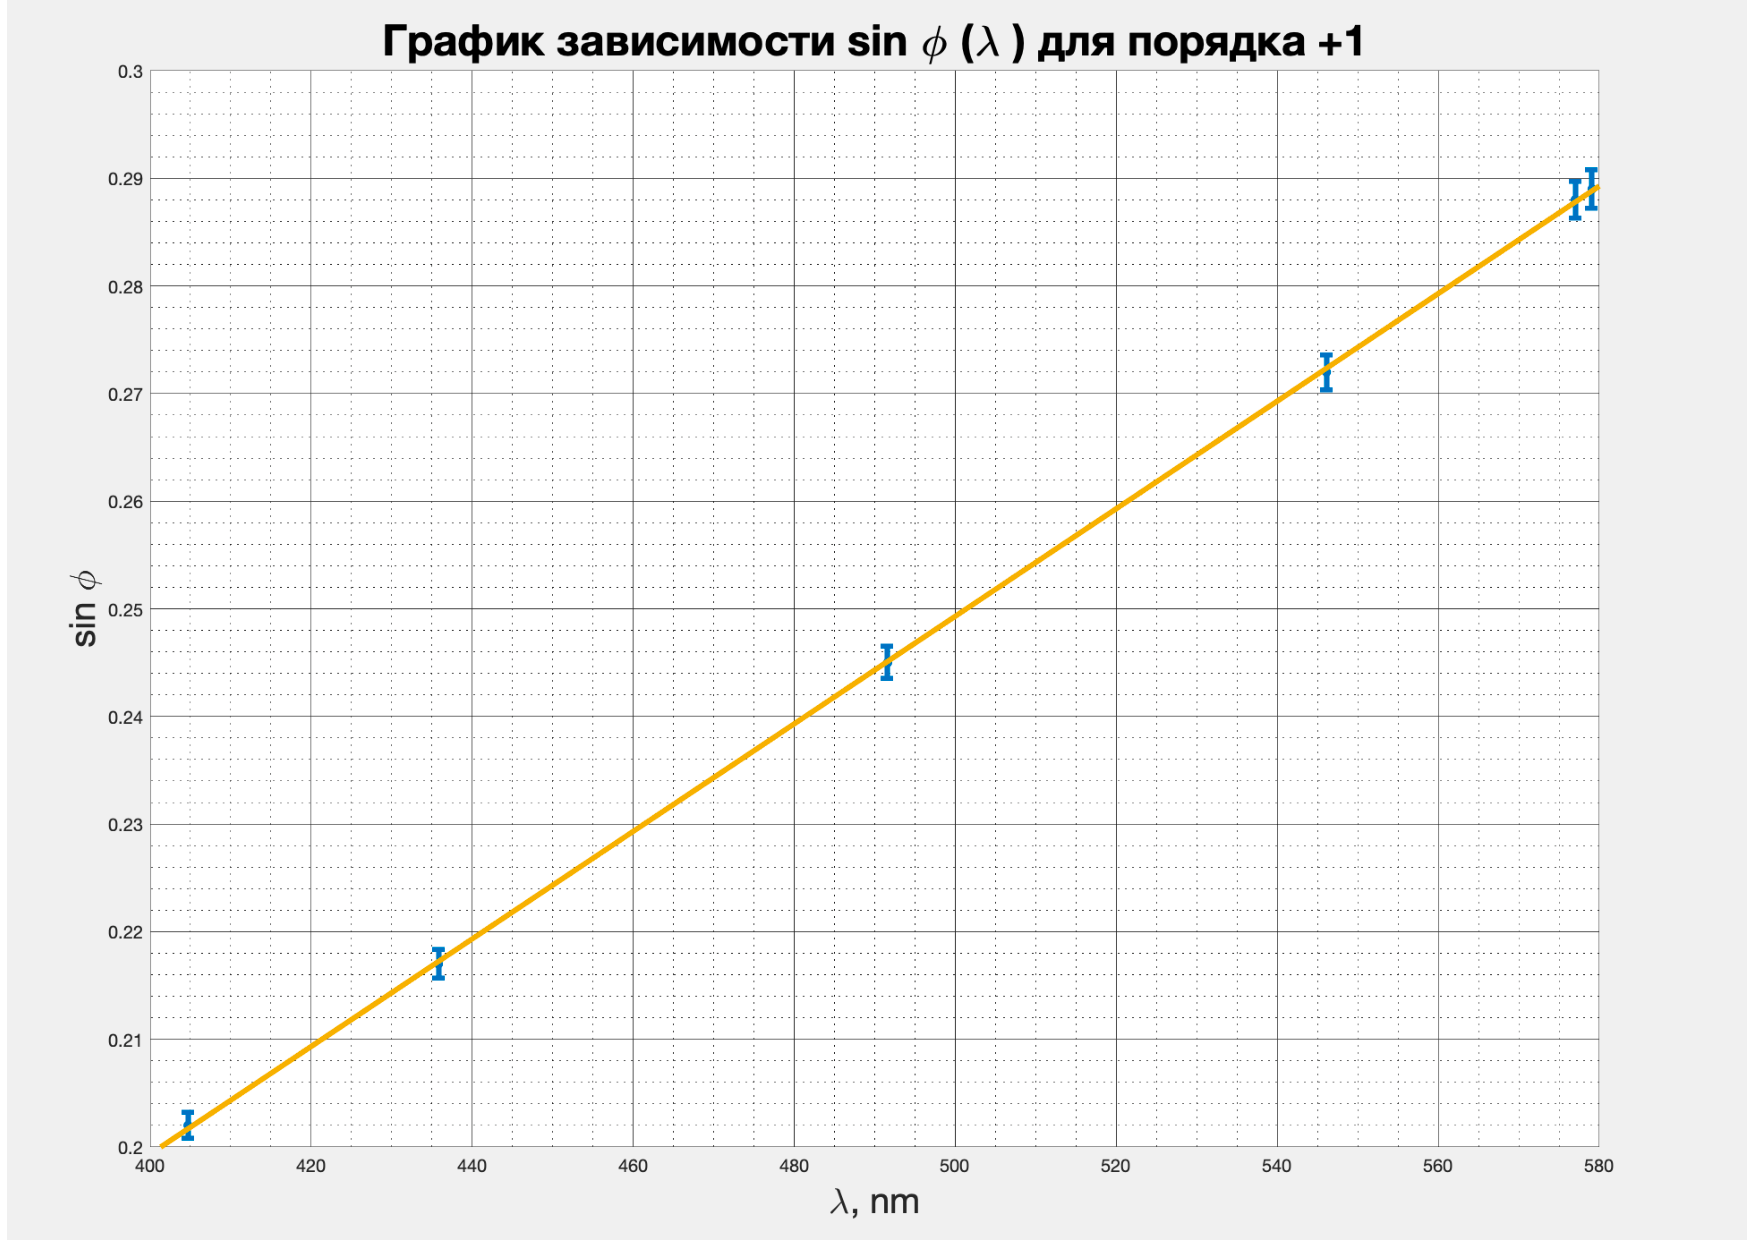
\includegraphics[width=0.72\linewidth]{gr1.pdf}
		\caption{график зависимости $\sin \varphi (\lambda)$ для 1-го порядка}
		\label{1st}
	\end{figure}
\end{center}


\begin{center}
	\begin{figure}[bhtp!]
		\centering
		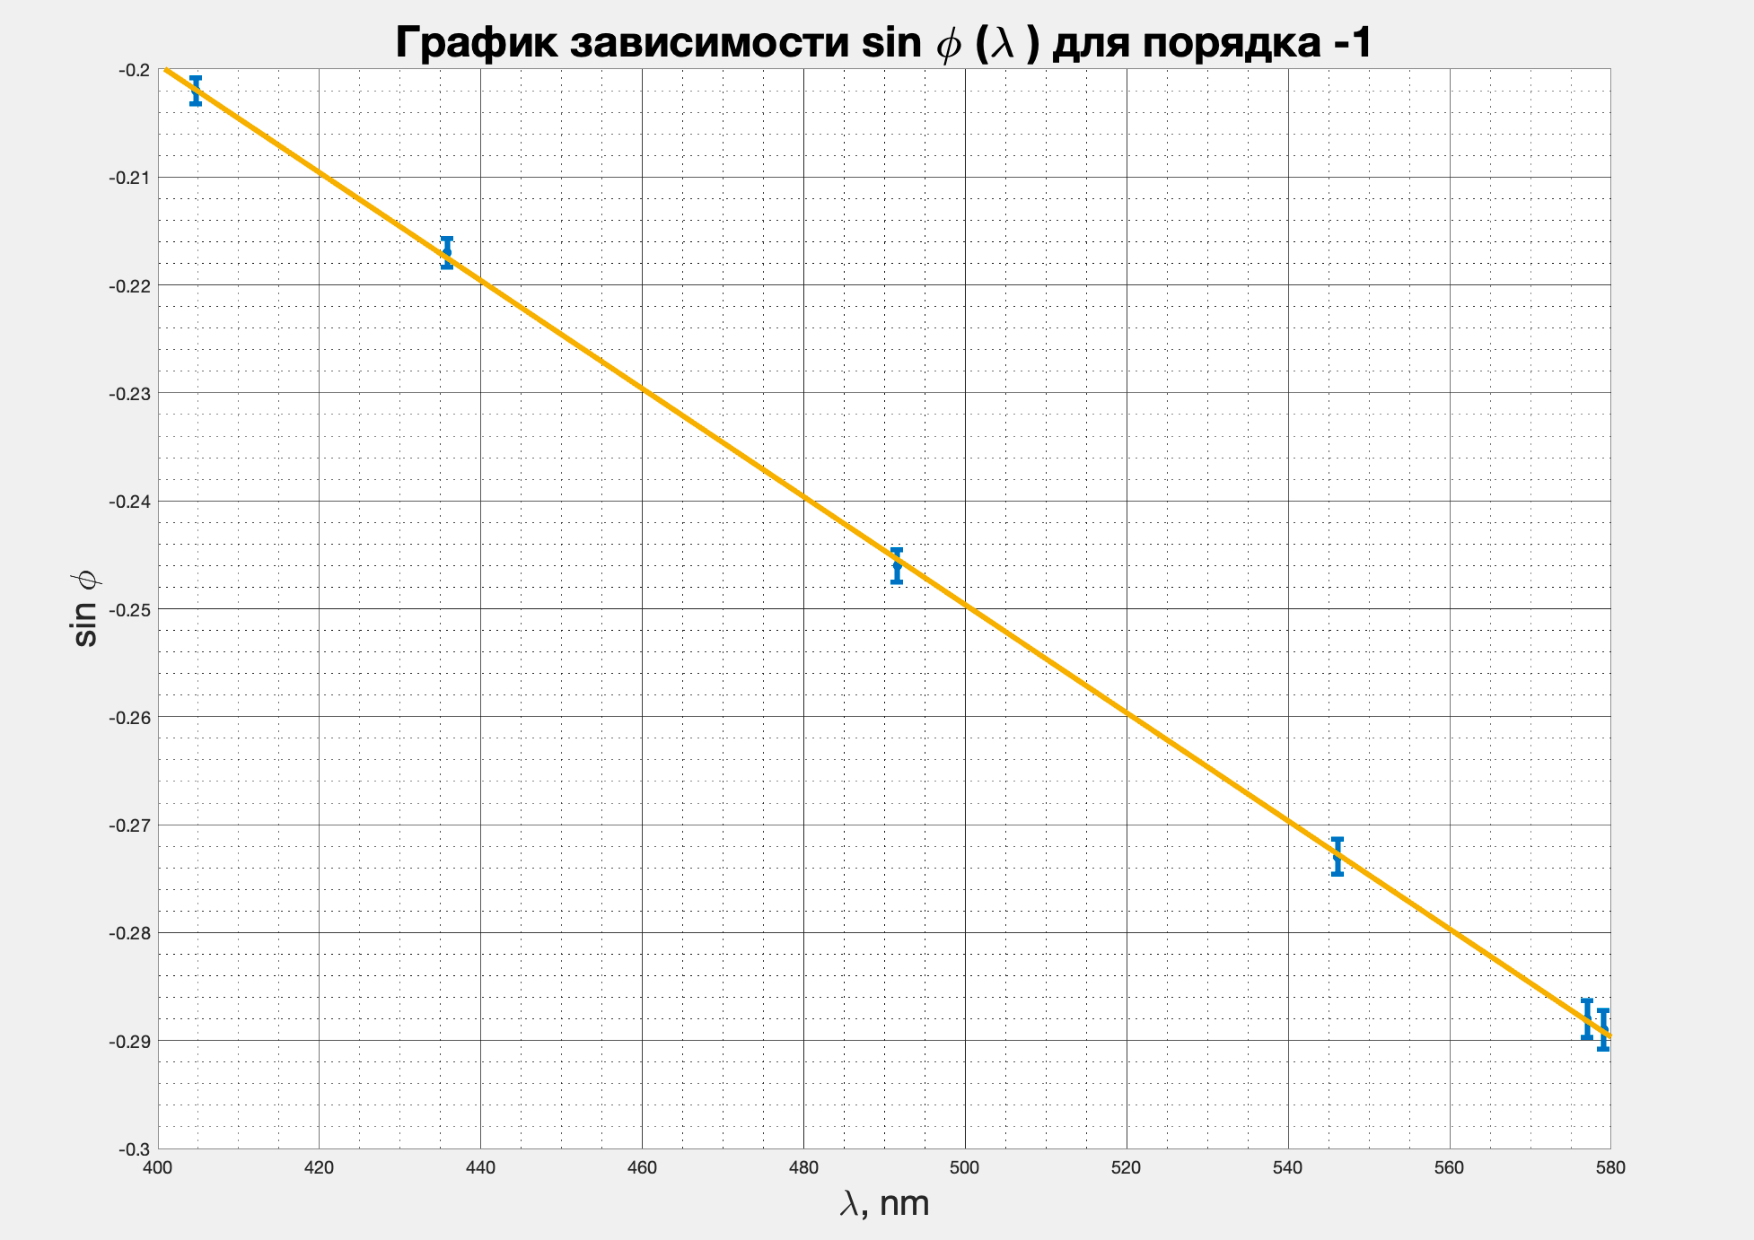
\includegraphics[width=0.72\linewidth]{gr2.pdf}
		\caption{график зависимости $\sin \varphi (\lambda)$ для -1го порядка}
		\label{-1st}
	\end{figure}
\end{center}
	
	
	\item Определим по графикам коэффициент наклона и с помощью него найдем шаг решетки:
	\[k_+ =  (2.00 \pm 0.03)\mkm \]
	\[k_- = (1.99 \pm 0.06)\mkm \]
	\[d = \pm \dfrac{\lambda}{\sin \varphi} \]
	Итого: $(d = 2.00 \pm 0.04)\mkm $
	
	\item Для оценки угловой дисперсии решетки определим угловые координаты линий желтой пары во всех видимых порядках спектра, положительных и отрицательных и занесём в таблицу $\ref{tabular:graph2}$
	
	
	\begin{table}[bhtp!]
		\begin{center}
			\begin{tabular}{|c|c|c|c|c|}
				\hline
				Цвет     & Порядок & $\varphi$ & $\Delta \varphi,~\text{угл. сек}$   & $D, \text{угл.сек/ангстрем}$  \\ \hline
				Желтый 1 & 1       & \ang{163;16;22} & 250  & 11.90  \\ 
				\cline{1-3}
				Желтый 2 & 1       & \ang{163;12;12} &   &  \\                     \hline
				Желтый 1 & -1      & \ang{196;45;9}  & -226 & -10.76 \\ 
				\cline{1-3}
				Желтый 2 & -1      & \ang{196;48;55} &  &  \\
				\hline
				Желтый 1 & 2       & \ang{144;47;50} & 576  & 27.43  \\ 
				\cline{1-3}
				Желтый 2 & 2       & \ang{144;38;14} &  &  \\ 
				\hline
				Желтый 1 & -2      & \ang{215;14;31} & -549 & -26.14 \\ 
				\cline{1-3}
				Желтый 2 & -2      & \ang{215;23;40} &  & \\
				\hline
			\end{tabular}
			\caption{угловые координаты линий желтой пары во всех видимых порядках спектра}
			\label{tabular:graph2}
		\end{center}
	\end{table}
	
	\item Рассчитаем экспериментальную угловую дисперсию для  желтой пары в  спектрах разных порядков по формуле:
	\[ D = \dfrac{\Delta \varphi}{\Delta \lambda}, \]
	где $\Delta \lambda = 21 \buildrel _{\circ} \over {\mathrm{A}}$.
	
	\item По полученным данным таблицы $\ref{tabular:graph2}$ построим график зависимости $D = f(m)$: см. рис. \ref{D(m)}
	
	\begin{center}
		\begin{figure}[bhtp!]
			\centering
			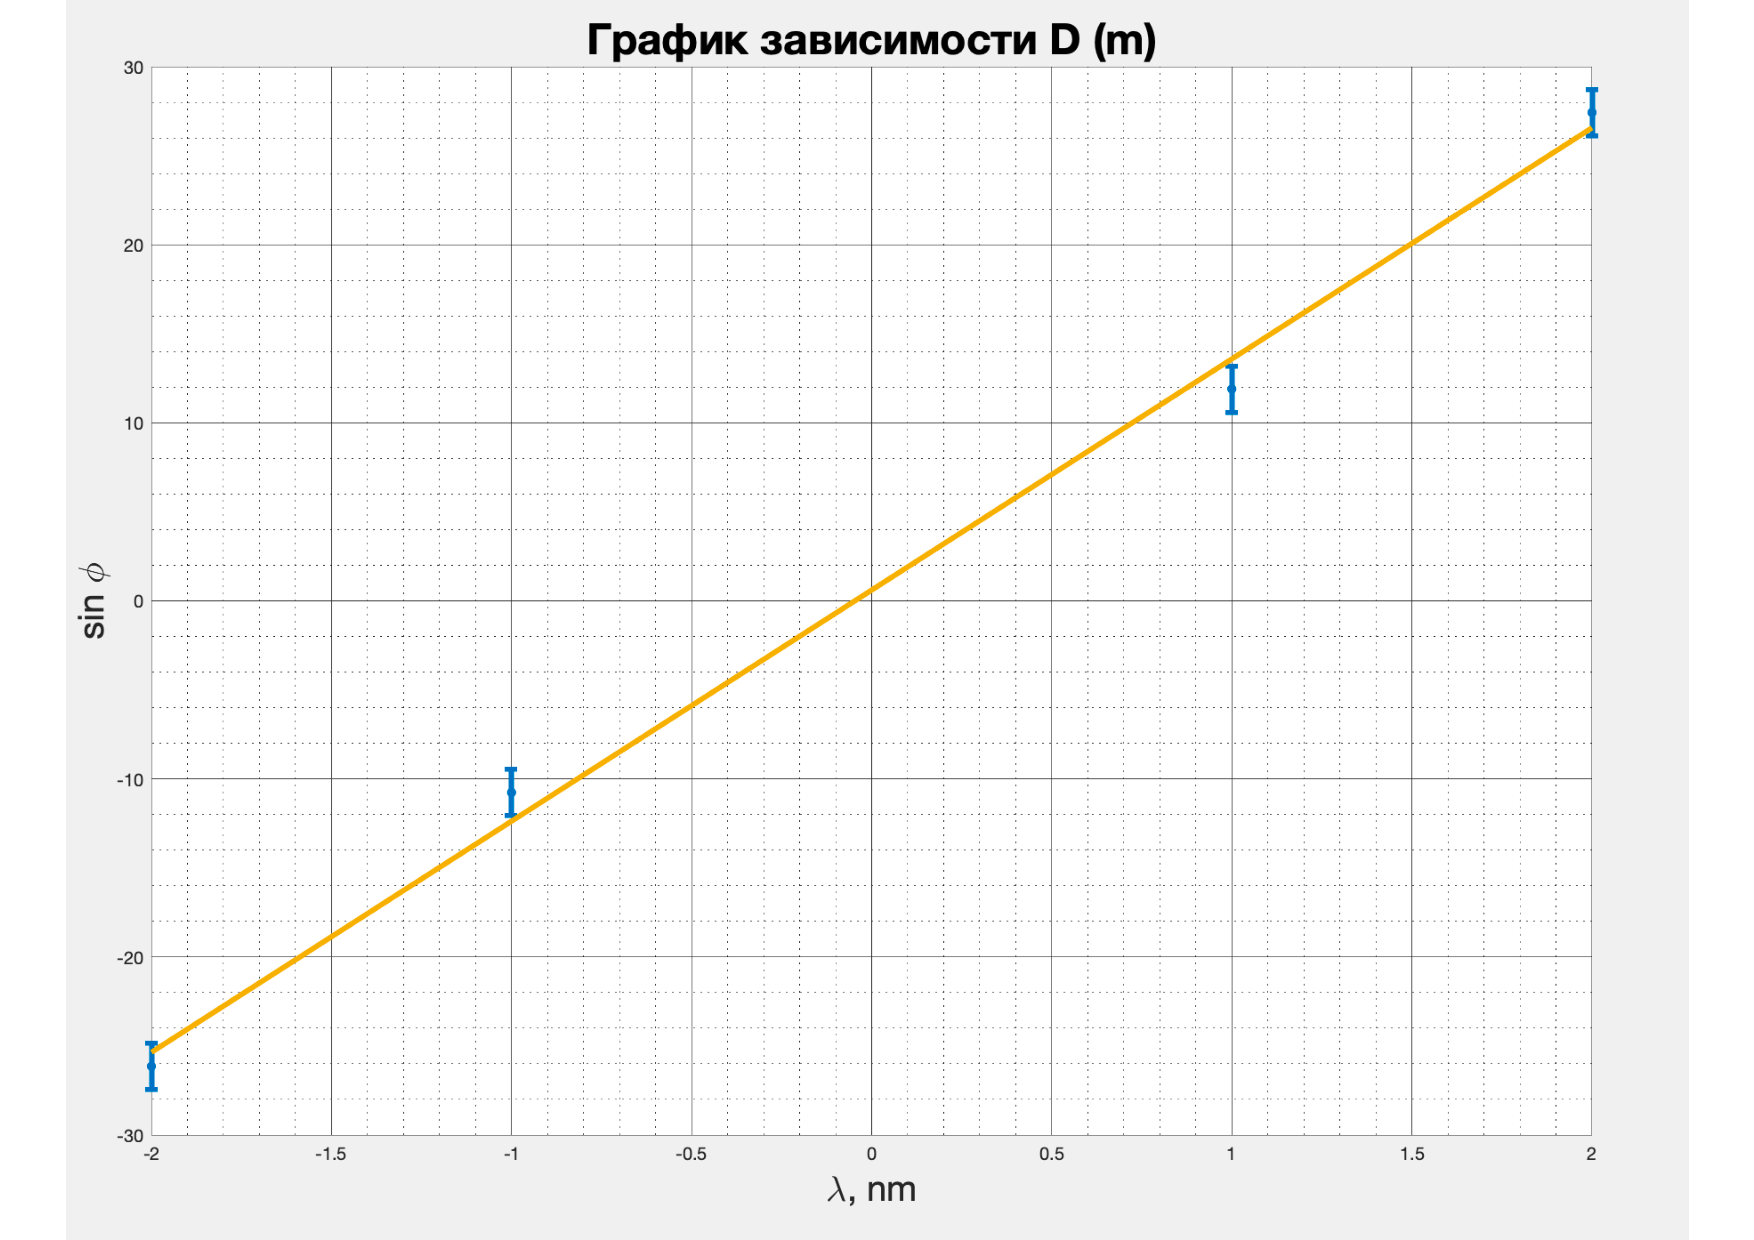
\includegraphics[width=\linewidth]{gr3.pdf}
			\caption{график зависимости $D = f(m)$}
			\label{D(m)}
		\end{figure}
	\end{center}
	
	\item По графику определяем коэффициент пропорциональности между $D$ и $m$:
	\[k_\text{эксп} = (12.9 \pm 0.6)~\text{угл.сек/ангстрем} = (0.63 \pm 0.03)~\mkm^{-1} \]
	\[k_\text{теор} \approx \dfrac{1}{d} = (0.50 \pm 0.02)~\mkm^{-1} \]
	
	\item Определим теоретическую разрешающую способность по формуле:
	\[R = \dfrac{\lambda}{\delta \lambda} = \dfrac{D\lambda}{\delta \varphi} = 274.8\]
	\item Сравнив её с теоретической, рассчитанной по формуле $R = mN$, оценим число эффективно работающих штрихов $N \approx 275$. Тогда размер освещенной части решетки~$\approx 0.55~\mm$.
	
	\item Рассчитаем порядок спектра, при котором фиолетовая линия наложится на желтую. Используя формулу $d \sin \varphi = m \lambda$, получаем
	\[ \dfrac{m_\text{ф}}{m_\text{ж}} = \dfrac{\lambda_\text{ж}}{\lambda_\text{ф}} = 1.43 \approx 10/7\]
	
\end{enumerate}

\section*{Вывод}

\noindent В ходе эксперимента мы ознакомились с принципами работы гониометра – оптического прибора для точного измерения углов. В результате измерения угловых координат спектральных линий ртути нашли экспериментально шаг решетки $d = (2.00 \pm 0.04)\mkm $, который довольно точно совпадает с приборным значением $d = 2~\mkm$.
С помощью измерения угловой полуширины желтого дублета, мы экспериментально нашли угловые дисперсии для разных порядков. И убедились в верности теоретической зависимости $D(m)$ для малых порядков.


\end{document}